\documentclass[a4paper]{article}

\usepackage{fullpage} % Package to use full page
\usepackage{parskip} % Package to tweak paragraph skipping
\usepackage{tikz} % Package for drawing
\usepackage{amsmath}
\usepackage{polski}
\usepackage[utf8]{inputenc}
\usepackage{booktabs}
\usepackage{subcaption}
\usepackage{hyperref}
\usepackage{amssymb}
\usepackage{amsmath}
\usepackage[ruled,vlined]{algorithm2e}
\usepackage{listings}

\usepackage[polish]{babel}
\usepackage{biblatex}
\addbibresource{references.bib}

\title{Kryptografia. Projekt.}
\author{Adrian Mucha, Mateusz Walczak}
\date{20. czerwca 2020}

\usepackage{graphicx}

\newtheorem{theorem}{Twierdzenie}

\begin{document}

\maketitle

\section{Wstęp}
Wybrane zadanie projektowe polegało na implementacji gry społecznościowej. W jej trakcie zadawane jest pytanie uczestnikom, na które mogą odpowiedzieć ,,tak'' lub ,,nie'', gdzie $x_i = 0$ oznacza, że $i$-ty uczestnik odpowiedział tak, w przeciwnym przypadku $x_i = 1$. Po odpowiedzi wszystkich uczestników podawana jest wiadomość, czy wszyscy odpowiedzieli twierdząco lub czy choć jedna osoba odpowiedziała negatywnie - zawetowała, co można zdefiniować, jako $max_i\{x_i\}$. Jednakże, pomimo poznania odpowiedzi zbiorczej gra musi zostać tak zaimplementowana, aby nie można było powiedzieć, kto jak głosował. Przedstawione zadanie jest przykładem tak zwanego problemu ucztujących kryptografów.

W poniższych sekcjach zostaną omówione pojęcia potrzebne do implementacji takiej gry i sam sposób.

\section{Problem ucztujących kryptografów} \label{section:dcProblem}
Problem ucztujących kryptografów został zaproponowany przez Davida Chauma na początku lat 80. poprzedniego wieku. Polega on na bezpiecznym obliczeniu funkcji $OR$ przez kilka niezależnych stron. 

Sytuacja została przedstawiona w formie historii, w której to trzech kryptografów siedzi przy okrągłym stole w restauracji. Po zjedzeniu kolacji kelner informuje ich, że ktoś zapłacił rachunek. Opłacającymi może być jeden z kryptografów albo NSA (ang. \textit{National Security Agency}). Kryptografowie szanują fakt, że jeden z nich mógł chcieć opłacić kolację anonimowo, jednakże chcieliby wiedzieć, czy przypadkiem to nie NSA opłaciło posiłek. 

\section{Sieć ucztujących kryptografów} \label{section:dcNetwork}
Jednym z rozwiązań problemu przedstawionego w sekcji \ref{section:dcProblem} jest sieć ucztujących kryptografów (ang. \textit{Dining Cryptographers network}). Schemat ten został zaproponowany przez Davida Chauma i składa się z dwóch etapów. Dla ułatwienia rozważmy taką sieć dla $3$ kryptografów.

W pierwszym etapie każda para kryptografów ustala wspólny jednobitowy sekret, na przykład poprzez rzut monetą. Nikt inny poza konkretną parą nie zna ich sekretu.

W etapie drugim każdy z kryptografów ogłasza jeden bit, taki że
\begin{itemize}
    \item jeśli nie zapłacił za posiłek jest to $XOR$ sekretów, które współdzieli ze swoim lewym i prawym sąsiadem,
    \item jeśli zapłacił jest to negacja funkcji $XOR$ sekretów, które współdzieli ze swoim lewym i prawym sąsiadem
\end{itemize}
Trzy tak ogłoszone bity następnie są ze sobą łączone za pomocą funkcji $XOR$. Dostawszy wynik wiadomym jest, czy któryś z kryptografów opłacił posiłek. Jeśli wynikiem jest $0$, wtedy za kolację zapłaciło NSA, w przeciwnym przypadku zrobił to kryptograf, jednakże jego tożsamość nie jest znana.

Na rysunku \ref{img:dcNetSimulation} przedstawione zostały dwa przypadki wykorzystania sieci ucztujących kryptografów, kiedy to jeden z kryptografów zapłacił i kiedy zrobiło to NSA.

\begin{figure}[h]
\centering
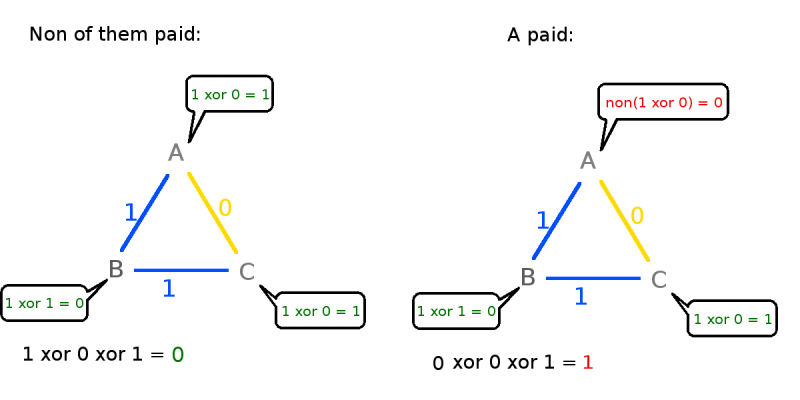
\includegraphics[width=0.8\textwidth]{images/Dinning_cryptographers.png}
\caption{Na diagramach kryptografowie zostali oznaczeni literami A, B i C. Współdzielone sekrety zostały oznaczone na liniach łączących litery. Diagram po lewej ilustruje sytuację, gdy NSA dokonało płatności, natomiast po prawej kolację opłacił kryptograf A. Źródło: \cite{dcSimulation}}
\label{img:dcNetSimulation}
\end{figure}

Sieć ucztujących kryptografów jednakże nie jest idealna. Przede wszystkim dla większej liczby kryptografów każdy z nich musi współdzielić sekret z każdym innym, co można zilustrować, jako graf pełny. Odbija się to na złożoności procesu. Co więcej, gdy do schematu zostanie dołączony kryptograf, który nie chce by inni poznali prawdziwą odpowiedź może to w łatwy sposób zrobić wysyłając losowy bit i nie zostanie to wykryte. Wartym zauważenia jest też fakt, że w tym schemacie używaliśmy ciągle funkcji $XOR$, co nie odpowiada na problem obliczania funkcji $OR$ przez kilka niezależnych stron, co zostało poruszone w sekcji \ref{section:dcProblem}.

\section{Anonimowe sieci wetujące} \label{section:avNetwork}
Konceptem, który rzeczywiście oblicza funkcję $OR$ i jest przystosowany do obsługi większej ilości użytkowników są anonimowe sieci wetujące zaproponowane przez Fenga i Zielińskiego w pracy \cite{avNetwork}. Nazwa anonimowych sieci wetujących (ang. \textit{anonymous veto network}) wzięła się od sytuacji, w której grupa uczestników dyskusji posiada prawo weta - powiedzenia ,,nie'', jednakże chcą to zrobić anonimowo.

Podobnie, jak w poprzedniej sekcji \ref{section:dcNetwork} przedstawmy model działania anonimowych sieci wetujących. Niech $n$ będzie liczbą uczestników. Następnie 
\begin{enumerate}
    \item uczestnicy zgadzają się na $(G, g)$, gdzie $G$ jest skończoną grupą cykliczną rzędu $q$, w której trudno jest rozwiązać problem DDH (ang. \textit{decisional Diffie-Hellman}). $g$ natomiast jest generatorem grupy $G$. 
    \item każdy z uczestników $P_i$ wybiera losową wartość $x_i$, taką że $x_i \in \mathbb{Z}_q$. Jest to jego sekret.
    \item rozpoczyna się pierwsza runda ogłaszania - każdy uczestnik ogłasza $g^{x_i}$
    \item po zakończeniu pierwszej rundy, to jest gdy każdy uczestnik ogłosi $g^{x_i}$, również każdy z nich oblicza $g^{y_i}$, gdzie
    \begin{equation}
        g^{y_i} = \frac{\prod_{j=1}^{i-1}g^{x_j}}{\prod_{j=i+1}^n g^{x_j}}  
    \end{equation}
    \item rozpoczyna się druga runda ogłaszania - każdy uczestnik ogłasza $g^{c_i y_i}$, takie że 
    \begin{equation}
        g^{c_i y_i} = 
        \begin{cases}
            g^{r_i y_i} & \quad \text{jeśli $P_i$ wysyła $1$, czyli weto}\\
            g^{x_i y_i} & \quad \text{jeśli $P_i$ wysyła $0$, czyli brak weta}
        \end{cases}
    \end{equation}
    , gdzie $r_i$ jest losową liczbą, taką że $r_i \in \mathbb{Z}_q$
    \item po ogłoszeniu przez wszystkich $g^{c_i y_i}$ można poznać wynik, czy ktoś zawetował poprzez obliczenie $\prod_i g^{c_i y_i}$.
\end{enumerate}
Jeśli nikt nie zawetował, wtedy $\prod_i g^{c_i y_i} = 1$, gdyż $\prod_i g^{c_i y_i} = \prod_i g^{x_i y_i}$, a $\sum_i x_iy_i = 0$. W przeciwnym wypadku $\prod_i g^{c_i y_i} \neq 1$. 

Wartym wspomnienia jest fakt, że dobrym kandydatem na grupę $G$ jest grupa Schnorra. Dodatkowo Feng i Zieliński w pracy \cite{avNetwork} podkreślają, że cały protokół odbywa się w czasie $O(n)$, liczba wysłanych danych może być określona, jako $O(n^2)$. Co więcej jest odporny na kolizje i zachowuje bezpieczeństwo semantyczne (ang. \textit{semantic security}), co zgodnie z pracą Fenga i Zielińskiego oznacza, że potencjalny obserwator nie może znaleźć różnicy pomiędzy $g^{x_i y_i}$ a $g^{r_i y_i}$.

\section{Grupa Schnorra} \label{schnorrGroup}
Grupa Schnorra jest podgrupą $\mathbb{Z}^*_p$ rzędu $q$, gdzie $q$ jest dużą liczbą pierwszą i $p$ również jest liczbą pierwszą. Do wygenerowania takiej grupy potrzebne są $p, q, r$, takie, że 
\begin{equation}
    p=qr+1.
\end{equation}
Następnie wybierane jest $h$, takie, że $1 < h < p$ oraz
\begin{equation}
    h^{r}\not \equiv 1\;({\text{mod}}\;p).
\end{equation}
Wartość $h^r$ jest równa 
\begin{equation}
    g=h^{r}{\text{ mod }}p,
\end{equation}
gdzie $g$ jest generatorem podgrupy $\mathbb{Z}^*_p$ rzędu $q$.

\section{TLS}
TLS (ang. \textit{Transport Layer Security}) jest rozwinięciem protokołu SSL (ang. \textit{Secure Socket Layer}). Zapewnia poufność i integralność transmisji danych, a także uwierzytelnienie serwera. W ramach protokołu TLS dostępne są algorytmy szyfrowania symetrycznego, jak i asymetrycznego. Składa się z następujących podprotokołów:
\begin{itemize}
    \item \textbf{Record Protocol} - przesyła dane w rekordach, które posiadająidentyfikator typu zawartości, mogą również skompresowane, zaszyfrowane i opatrzone w kod MAC
    \item \textbf{Handshake Protocol} - inicjalizuje połączenie, negocjuje klucze i transformacje kryptograficzne
    \item \textbf{Change Cipher Spec} - zmienia ustalone parametry kryptograficzne
    \item \textbf{Alert Protocol} - powiadamia o powstałych błędach
\end{itemize}

Wartym dodania jest fakt, że do uwierzytelniania serwera w protokole TLS wykorzystywane są certyfikaty. Certyfikat zawiera m.in. domenę, dla której został wystawiony. Wystawiane są przez urzędy certyfikacji (ang. \textit{Certificate authority}), które są specjalnymi instytucjami weryfikującymi, czy dana domena może posługiwać się danym certyfikatem.

Dodatkowo istotną kwestią całego protokołu są klucze wykorzystywane w algorytmach szyfrowania, a dokładnie ich długość, bo to ona odpowiada za bezpieczeństwo protokołu. Zalecaną długością dla kluczy asymetrycznych jest 2048 bitów, natomiast dla symetrycznych długość 128 lub 256 bitów.


\section{Implementacja systemu}
System, który pozwala na przeprowadzenie w grupie użytkowników głosowania składa się z dwóch części - serwerowej i klienckiej. Cały system implementuje koncept anonimowych sieci wetujących, które zostały omówione w sekcji \ref{section:avNetwork}. Komunikacja pomiędzy nimi odbywa się za pomocą protokołu TLS.

    \subsection{Część serwerowa}
    Do jej stworzenia został wykorzystany język \texttt{Javascript}, środowisko \texttt{Node.js} w wersji \texttt{14} oraz biblioteka \texttt{express} w wersji \texttt{4.16.1}. 
    
    Część serwerowa umożliwia stworzenie grupy składającej się z $n$ członków i pytania. Podczas tworzenia takowej grupy tworzone jest jej $id$, które później pozwoli innym użytkownikom odpowiadanie na pytanie oraz grupa $G$ i jej generator $g$. Grupa $G$ jest grupą Schnorra dla $r = 2$, tzn. jest grupą reszt kwadratowych modulo bezpieczna liczba pierwsza, czyli taka, że jest równa $2q + 1$, gdzie $q \in PRIME$. Liczba $q$ generowana jest za pomocą programu \texttt{openssl}. Mając $p, q, r$ grupa $G$  i generator $g$ są generowane jest zgodnie z algorytmem podanym w sekcji \ref{schnorrGroup}.
    
    Część serwerowa umożliwia również ogłaszanie swoich kluczy $g^{x_i}$ i zapamiętuje je. 
    
    W momencie zebrania wszystkich kluczy, tj. $n$ kluczy serwer umożliwia zagłosowanie użytkownikom poprzez przesłanie wartości $g^{c_i * y_i}$. Wartości te zapisywane są na serwerze, w momencie zebrania wszystkich odpowiedzi, tj. $n$, klient jest w stanie odczytać odpowiedzi i obliczyć wynik, czy ktoś zawetował w głosowaniu.
    
    \subsection{Część kliencka}
    Do zaimplementowania części klienckiej wykorzystany został język \texttt{Python} w wersji \texttt{3.8.0} oraz biblioteka \texttt{requests} w wersji \texttt{2.24.0}. 
    
    Część kliencka symuluje zachowanie klienta. Takich symulacji zostanie uruchomionych $n$, z czego tylko jedna będzie tworzyć grupę z pytaniem. Po otrzymaniu parametrów grupy $G$, to jest mając generator $g$ oraz rząd $q$ wybierze $x_i$ i wyśle do serwera klucz $g^{x_i}$.
    
    Następnie klient będzie sprawdzał odpytując serwer, czy wszystkie $n$ kluczy jest dostępne. W momencie kiedy serwer zwróci pełną listę natychmiast oblicza $g^{y_i}$ i oddaje głos za lub przeciw w zależności od parametrów uruchomienia. Głos jest oddawany również przez wysłanie danych na odpowiedni endpoint serwera. 
    
    Na koniec klient podobnie, jak dla kluczy odpytuje serwer o informacje na temat odpowiedzi, czy wszyscy już jej udzielili. W momencie gdy lista odpowiedzi jest pełna wylicza, czy ktoś zawetował i wypisuje informację o przebiegu głosowania. 
    
\clearpage
\printbibliography

\end{document}
